\chapter{Usage}\label{Usage}
This chapter will describe the systems interaction with its surroundings. This will be done by making an actor specification and then presenting user pattern diagrams, which will be showcased in state machines.

\section{Actor specification}
\label{Actor_specification}
An actor will be described by an actor specification , the actor is a user of the system.

\hrule
\begin{tightcenter}
\textit{\textbf{User}}
\end{tightcenter}
\hrule
\textbf{Objective:} A person who prepare their meals themself, either for themself or for a household. The user's primary need is to plan their week in order to efficiently shop their groceries and lessen food waste.\\

\textbf{Characteristic:} The system includes a user base of which the users have different needs and preferences.

\textbf{Example one:} User A is an allergy sufferer and has to make meals which excludes nuts. When A is shopping she needs to look at the package info to make sure that the product does not contain trace of nuts.

\textbf{Example two:} User B is a young student who is in a relationship. User B has a tight budget and a little time frame to shop in. B finds it difficult to sustain an overview of their share storage of food. Therefore B will sometimes buy products they do not need, for example, B might purchase milk even though they already have three litres stored. This will sometime result in them not being able to use all the milk before it expires, which is bad for their shared budget and food waste.
\hrule



\section{User pattern}
The user pattern shows an abstraction between the interactions in the system and actor. State machine diagrams are used to show these interactions. The diagrams show how the dynamic states can shift trough interactions with the actor. Even though many of the details is excluded, it still gives a good overview of how the logic is set up in the user pattern and how the the dynamic flow goes. 

The purpose of the diagram is to create an overview of the application domain's interactions with the system. This will be used to find acquirements for the functions and user interface. There are three user pattern diagrams, each representing different areas of the system. The three diagrams showcase the user patterns in the:
\begin{itemize}
\item{Shopping list}
\item{Foodplan}
\item{Inventory}
\end{itemize}

When the user actor traverses trough the system, the actor will undertake one of two roles. An administrative or a planning oriented role.
The option to go back or cancel have not been drawn on the diagrams as their only contribution is to make the diagrams less readable and add redundant repetitions, that goes for all of the diagrams.

%\begin{figure}[H]
%	\centering
%	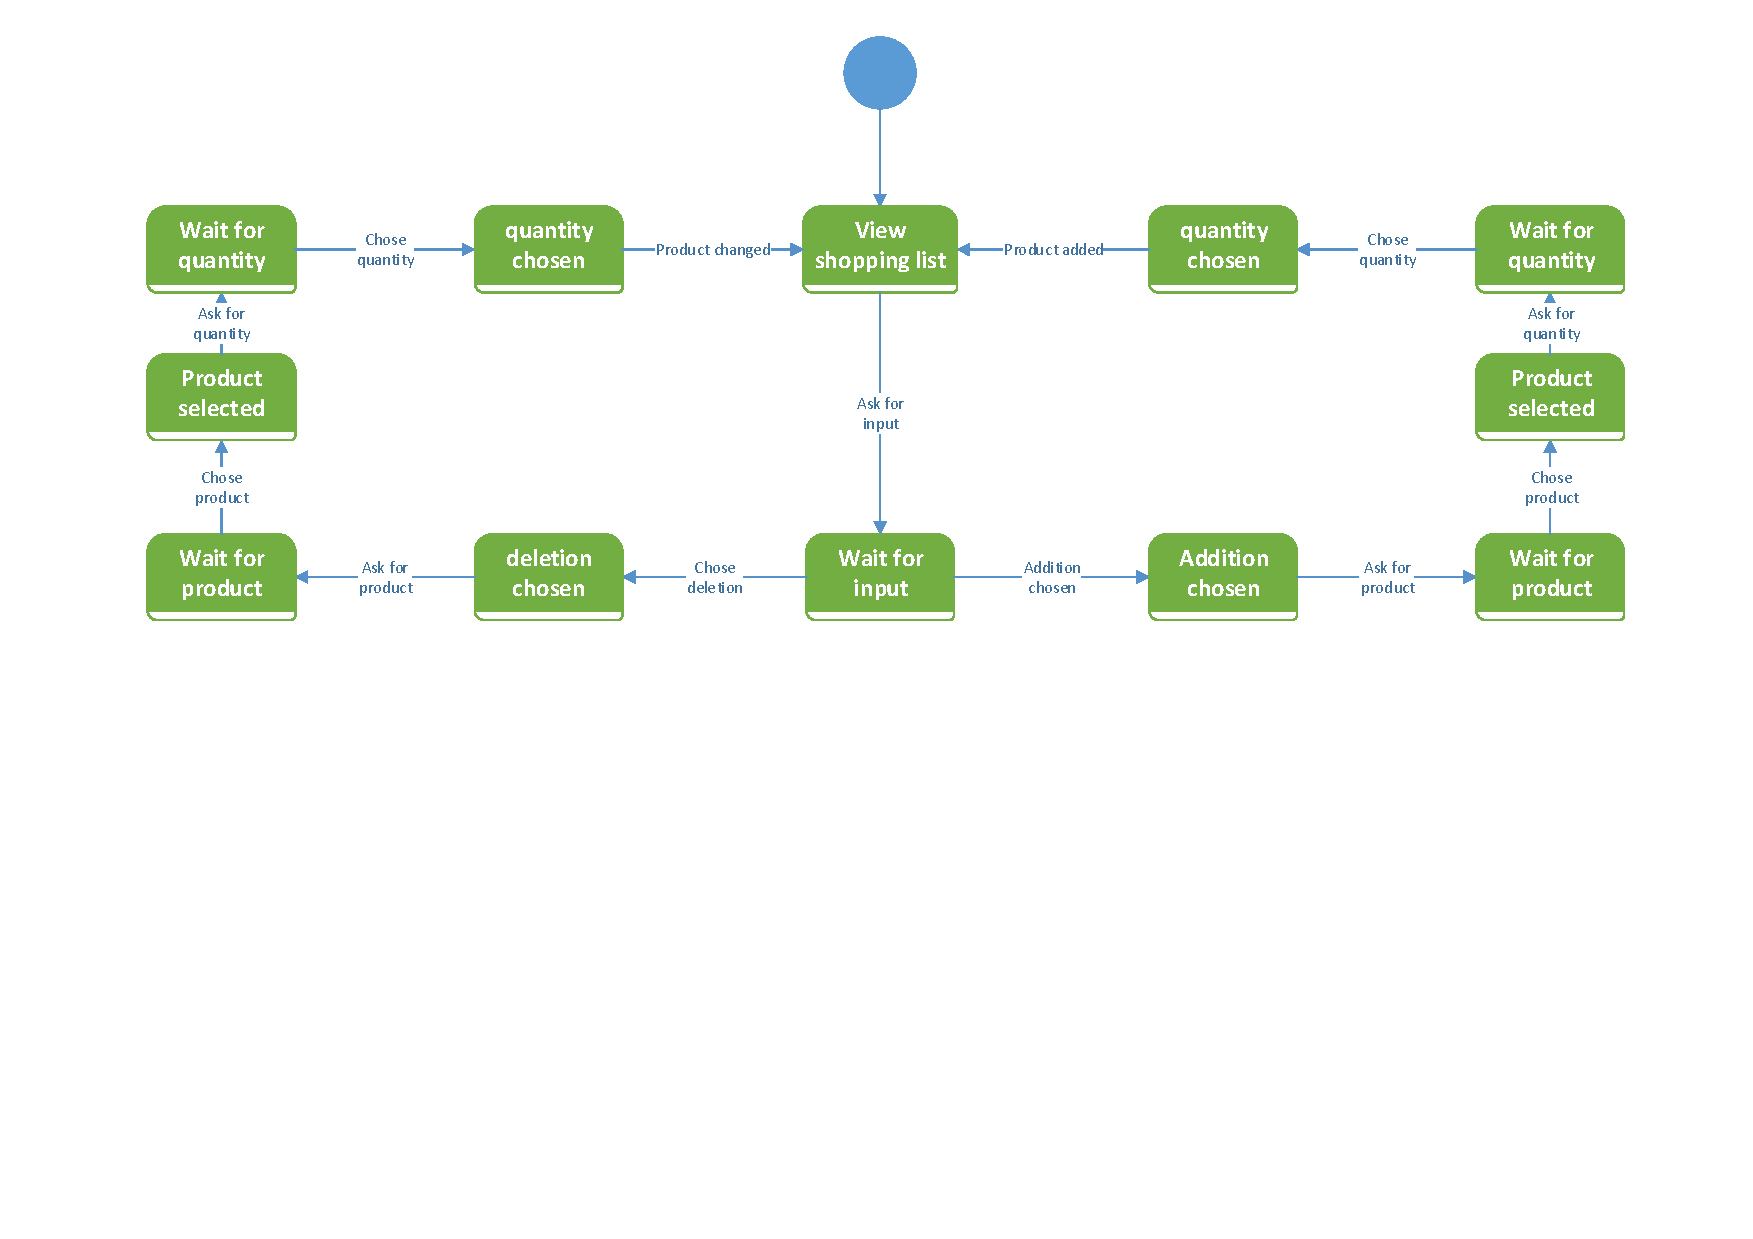
\includegraphics[width=1.0\textwidth]{ApplicationDomain/upShoppingList.pdf} 
%	\caption{The view shopping list state diagram}
%	\label{Shopping_List_Figure}
%\end{figure}
%When the user goes to the shopping list, the program will wait for him to either add or delete an product. If he chooses to add a product to the list, he will be asked to chose a product. The product also needs a quantity that specifies how much of the product is needed to be listed (2 litres of milk or ½ kilo of flour). If an valid quantity is given it will be added to the shopping list an the user will be able to add or delete another product. The only quantity that is not acceptable is value that is below or equal to zero.
%
%The user is also able to delete a product from the shopping list. The user will then have to chose an item already present on the list and then chose how much of the product tat should be removed from the list. If the user chooses a quantity that will leave the product at a zero quantity the product will be removed altogether from the list. For example if the list contains four apples, and the user removes three apples, one apple will still be present on list. However, if the user decided to remove four apples, the list will no longer contain the product apples. It should be noted that trying to remove a quantity of a product that will leave i a negative value will result in an error.

This diagram is for the foodplan, in this part of the system the user actor operates under the planing role.

\begin{figure}[H]
	\centering
	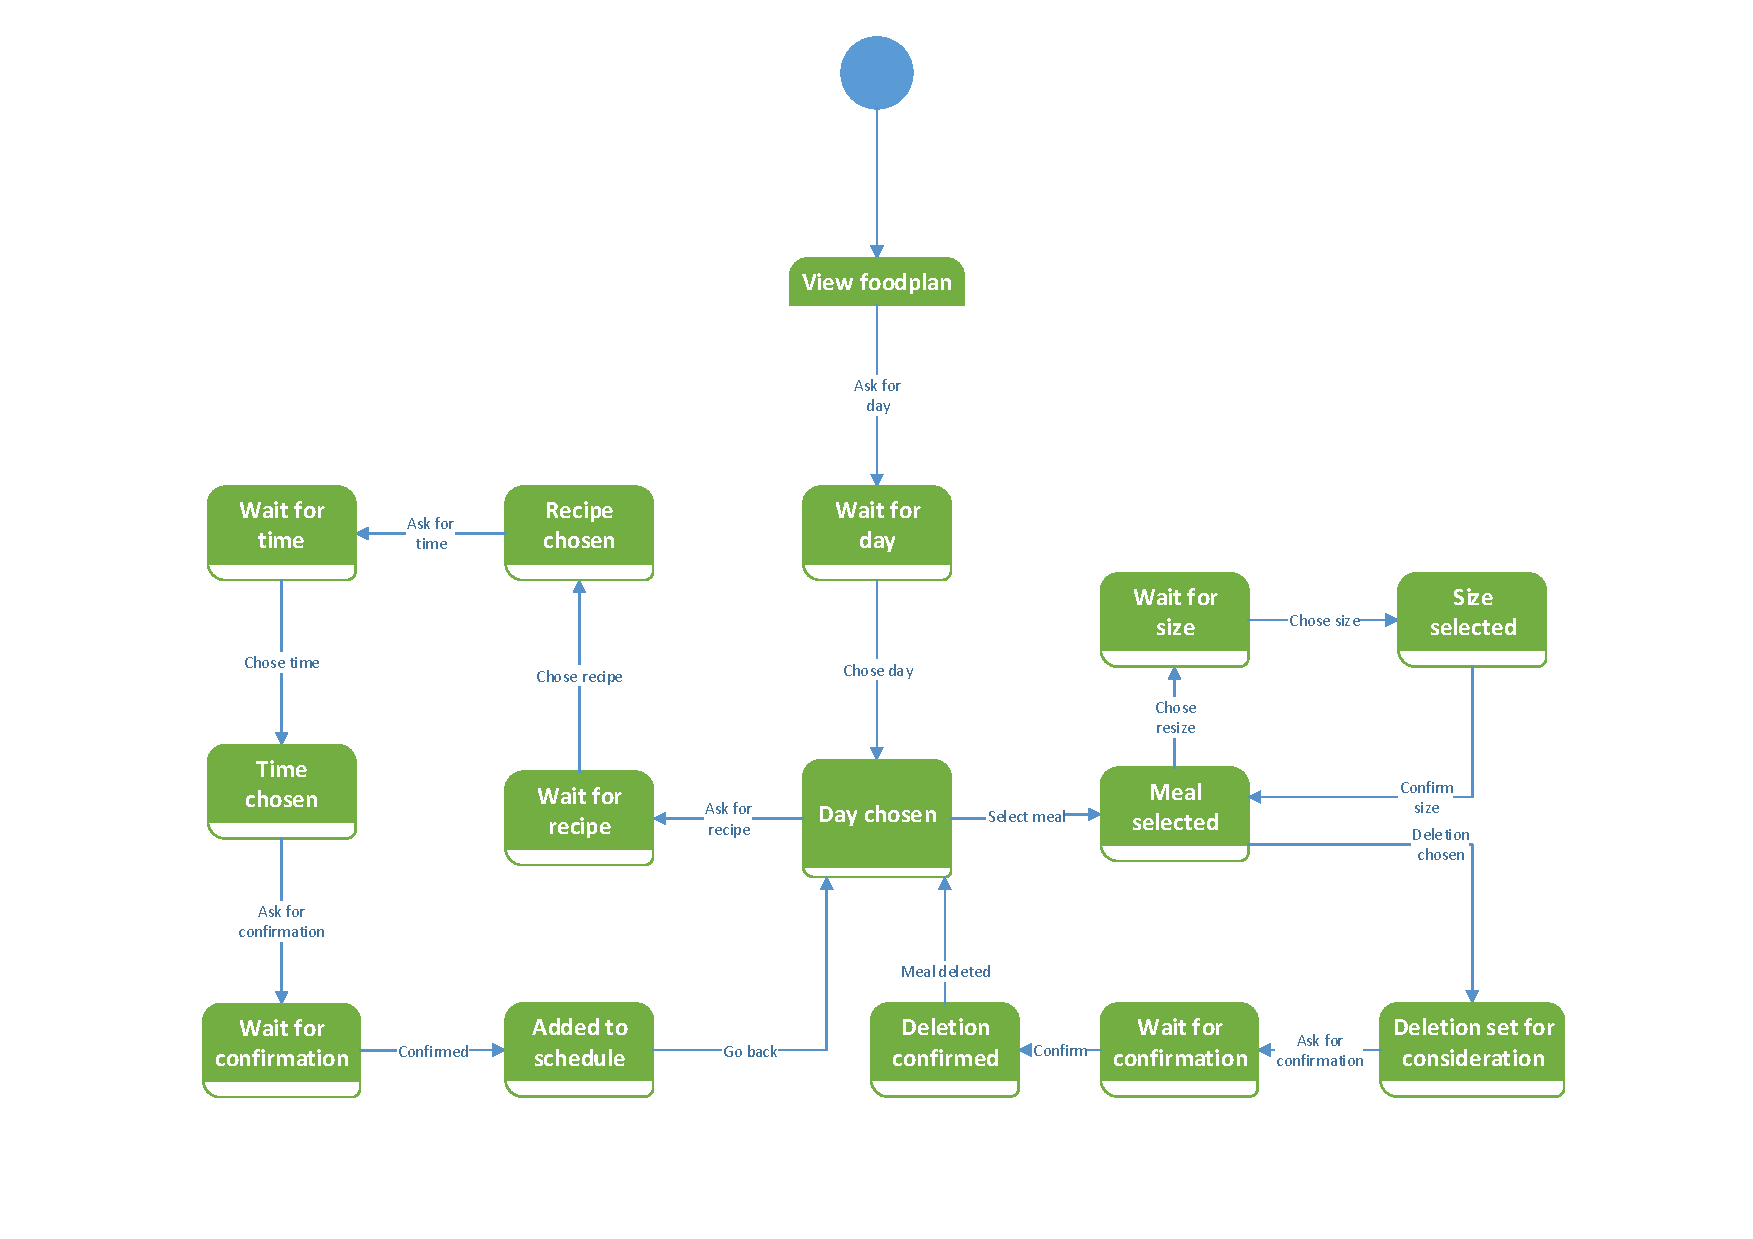
\includegraphics[width=1.0\textwidth]{ApplicationDomain/spViewFoodPlan.pdf} 
	\caption{The view foodplan state diagram}
	\label{Foodplan_Figure}
\end{figure}
When the user goes to the foodplan part of the system, he will have to choose a day to view the foodplan for. From there the user can add a new meal to the plan or select an existing planned meal. If the user chooses to add a new meal, the system will ask for a recipe. The recipes the user can choose from varies depending on the user's preferences. If the user have chosen to avoid some products, recipes that contain those products will be excluded. When a recipe have been chosen, a time for when on the day the meal should be prepared for will have to be entered. After the time has been entered, the meal will be added to the schedule.


The next two diagrams is for the inventory. In this part of the system the actor operates as a administrator.

\begin{figure}[H]
	\centering
	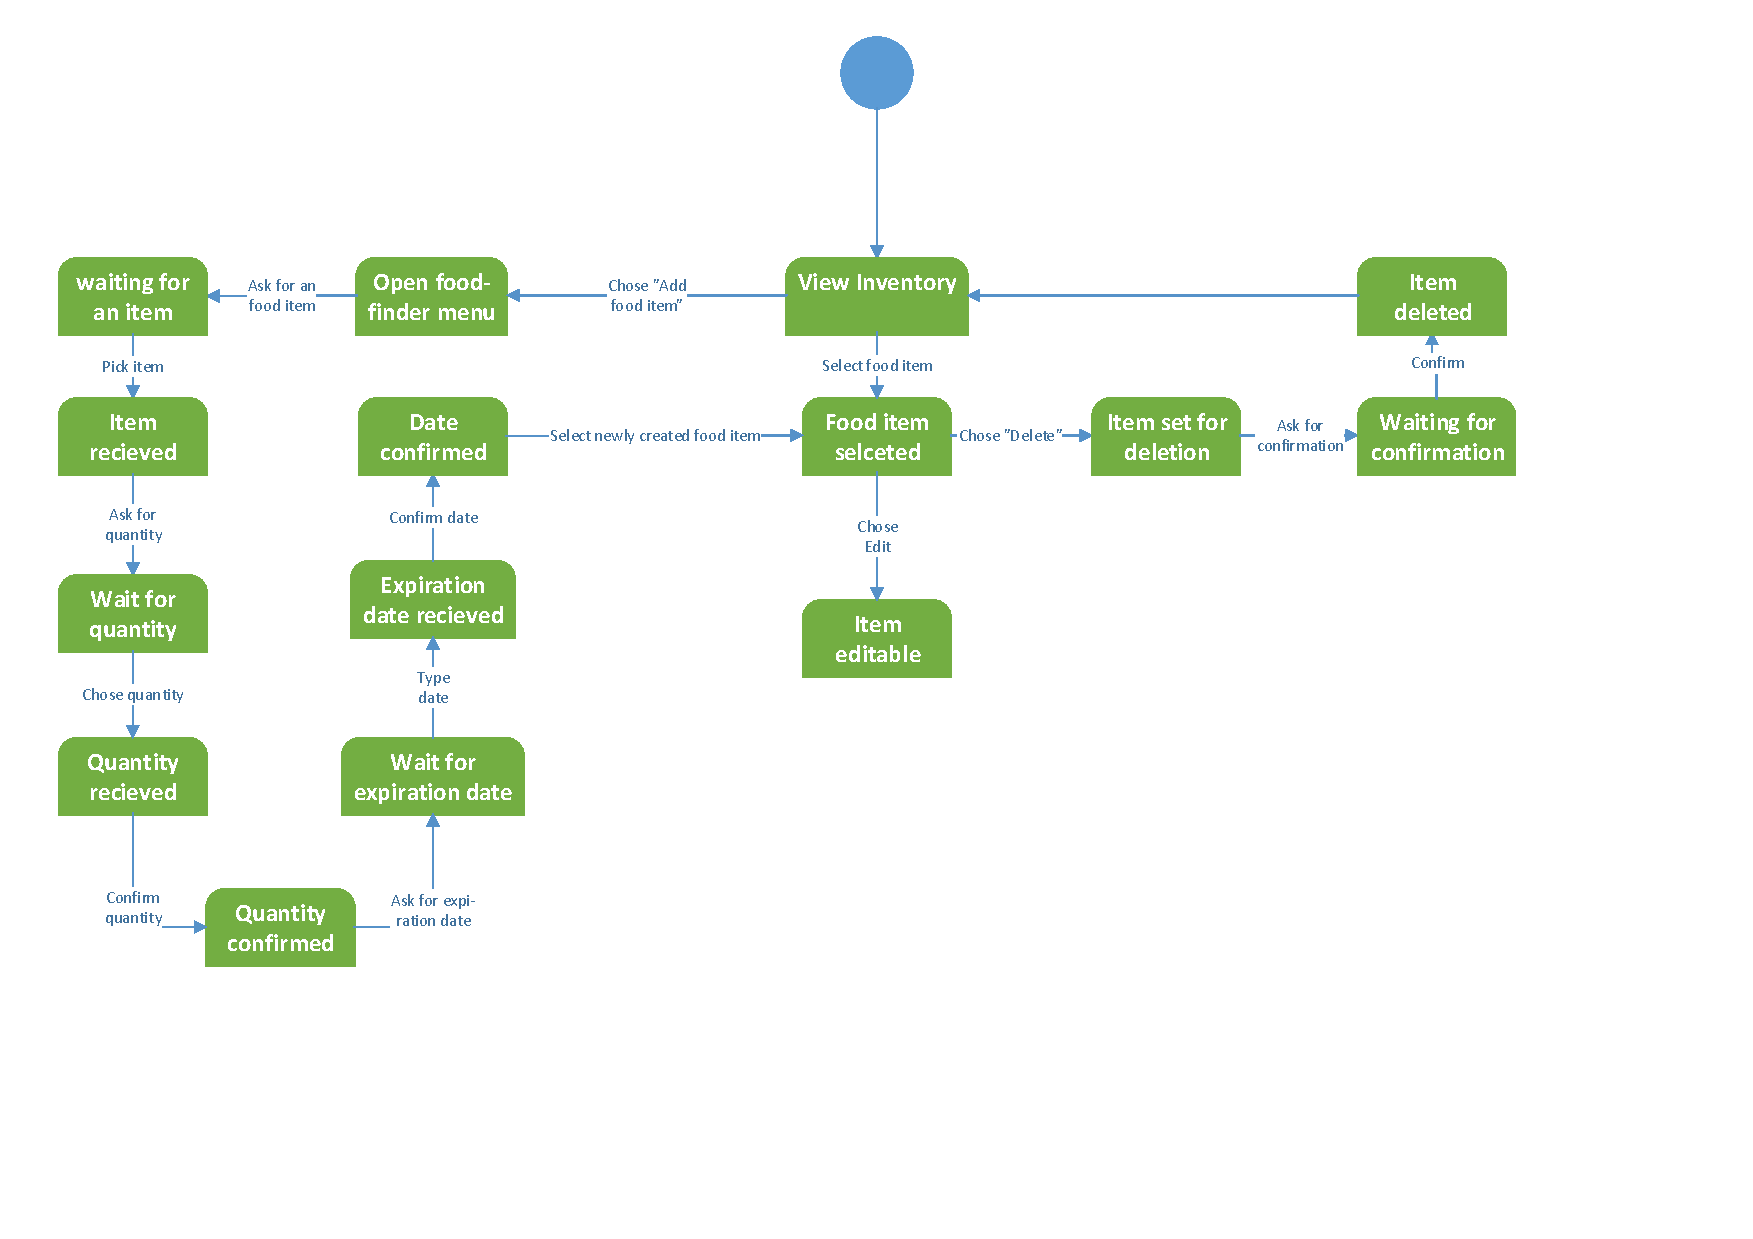
\includegraphics[width=1.0\textwidth]{ApplicationDomain/spViewInventory.pdf} 
	\caption{The \textit{view inventory} state diagram}
	\label{Inventory_Figure}
\end{figure}
The user starts out on the "view inventory" state where the inventory is shown. From here the user can choose from three different options: One that adds food to the inventory, another which allows the user to delete existing food items and a last option for editing food items. The edit option has its own diagram (see \cref{spEditInventory}). If the user chooses to add food, they will have to select food from a food list. When a food item have been chosen, the system will ask for the user to select an quantity in order to know how much of the food item the user have acquired. For example, the user can buy five bananas or two hundred grams of flour. The user will afterwards have to enter when the food expires. When this is done the food will be added to the inventory. This leaves the user at the food item they have added, as if it were selected on the inventory screen. This is the same result as if the user chose to select an food item from the beginning. From here the user will be able to edit or delete an food item. \label{InvDesc}

When the user chooses to delete a selected item the system will ask for an confirmation for that user wanted to delete. If the user confirms, the system will delete the food item and go back to the view inventory state.


The following diagram, is the last diagram which also covers the inventory. In this part of the system the actor operates as a administrator.

\begin{figure}[H]
	\centering
	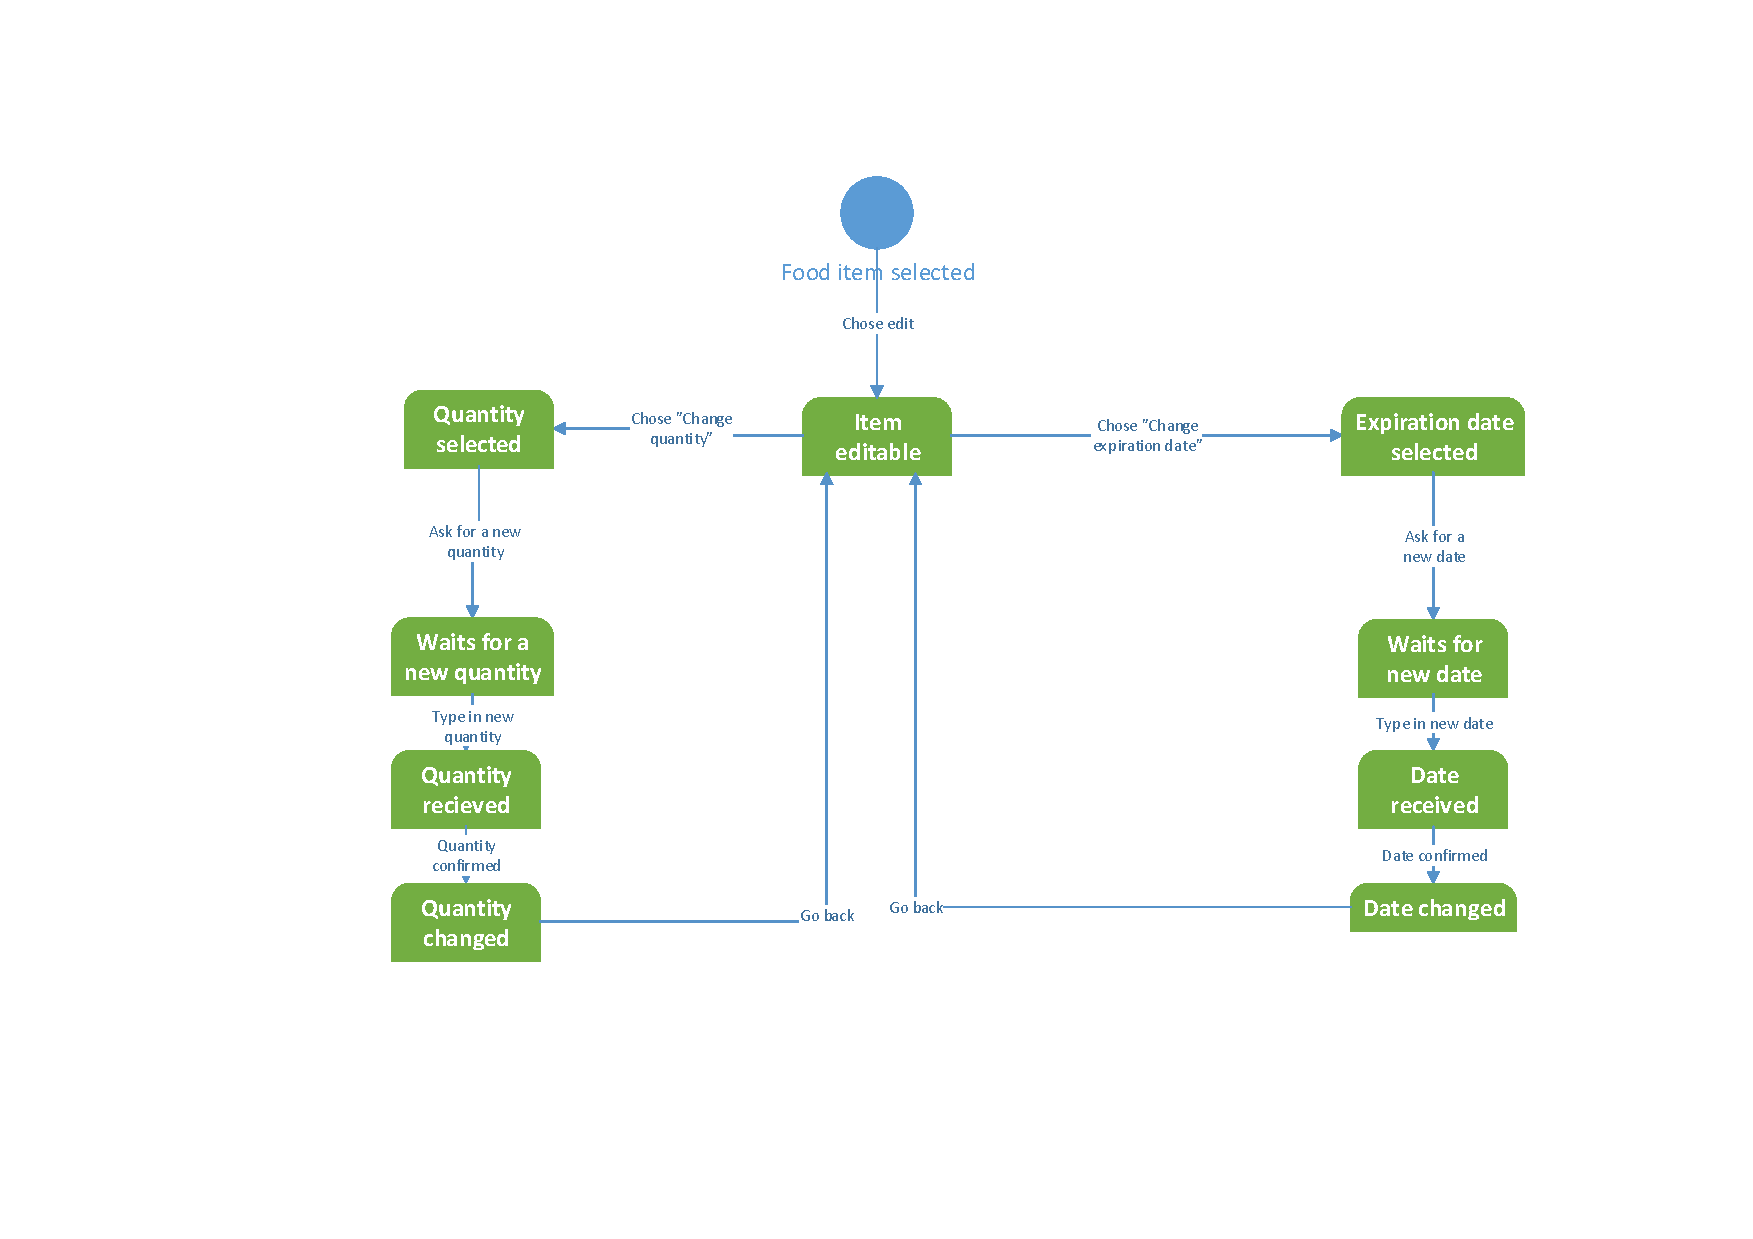
\includegraphics[width=1.0\textwidth]{ApplicationDomain/spEditInventory.pdf} 
	\caption{The edit inventory state diagram}
	\label{spEditInventory}
\end{figure}
The possible options in form of editing is to change the quantity or expiration date. 
When choosing \textit{Change quantity} it works like the \textit{Change quantity} in the shopping list, which means that choosing an amount that leaves it at zero deletes the item, and leaving it below zero result in an error. When the user tries to change the expiration date, the system prompts for a new date. All dates will be valid, which means that an item which was expired can go "unexpired" as described at the diagram \cref{MealClass}. This also works the other way around as an fresh item can expire if the date changes to the day prior to the day it expires.


\section*{Summary}
The actor specification helped to establish a understanding of how the user base will interact with the system. The user patterns helped to reinforce that understanding. By making the user patterns, some flaws in the design were discovered which resulted in varies tweaks and reworks.\fxnote{Skal vi have sidste sætning med, når vi ikke har beskrevet disse fejl?}